\chapter{Uitwerken prototype ---GEKOZEN FRAMEWORK---}
\label{ch:prototype}

Dit hoofdstuk bevat een omschrijving van het uitgewerkte prototype. Het prototype bestaat uit verschillende grote delen die elk besproken worden in een aparte sectie.

\section{Unity Asset Store}
Unity beschikt over een Asset Store die developers, designers en zelfs muzikanten kunnen gebruiken om hun werk te delen met anderen. De assets op deze store kunnen andere developers dan gebruiken in hun projecten. Voor de ontwikkeling van het protype zijn volgende assets gebruikt:

\begin{itemize}
    \item ZoneUI (INSERT LINK)
    \item Clean Title Transitions (INSERT LINK)
\end{itemize}

\section{Hoofdmenu}
Wanneer de gebruiker de applicatie opstart komt hij op de hoofdpagina terecht. Op deze pagina heeft hij verschillende opties waaruit hij kan kiezen. Als het de gebruiker zijn eerste keer is dat hij de applicatie gebruikt zullen alleen de opties 'Nieuw Levensverhaal' en 'Oud Levensverhalen bekijken' beschikbaar zijn. Indien de gebruiker toch al eens de applicatie heeft opgestart kan hij verder doen met zijn recentste levensverhaal of kiezen uit één van zijn niet voltooide levensverhalen. 

Vanuit het hoofdmenu heeft de gebruiker ook nog de optie om naar de instellingenpagina te gaan of naar zijn profielpagina. Op de gebruiker zijn profiel staan verschillende weetjes zoals het aantal deelgenomen levensverhalen, voltooide raadsels en ontdekte schilderijen. Ook heeft de gebruiker een level dat berekent is aan de hand van deze variabelen. Het behalen van een bepaald level is momenteel puur aesthetic en zit in de applicatie om de gebruiker een gevoel van trots en prestatie te geven.

\begin{figure}
    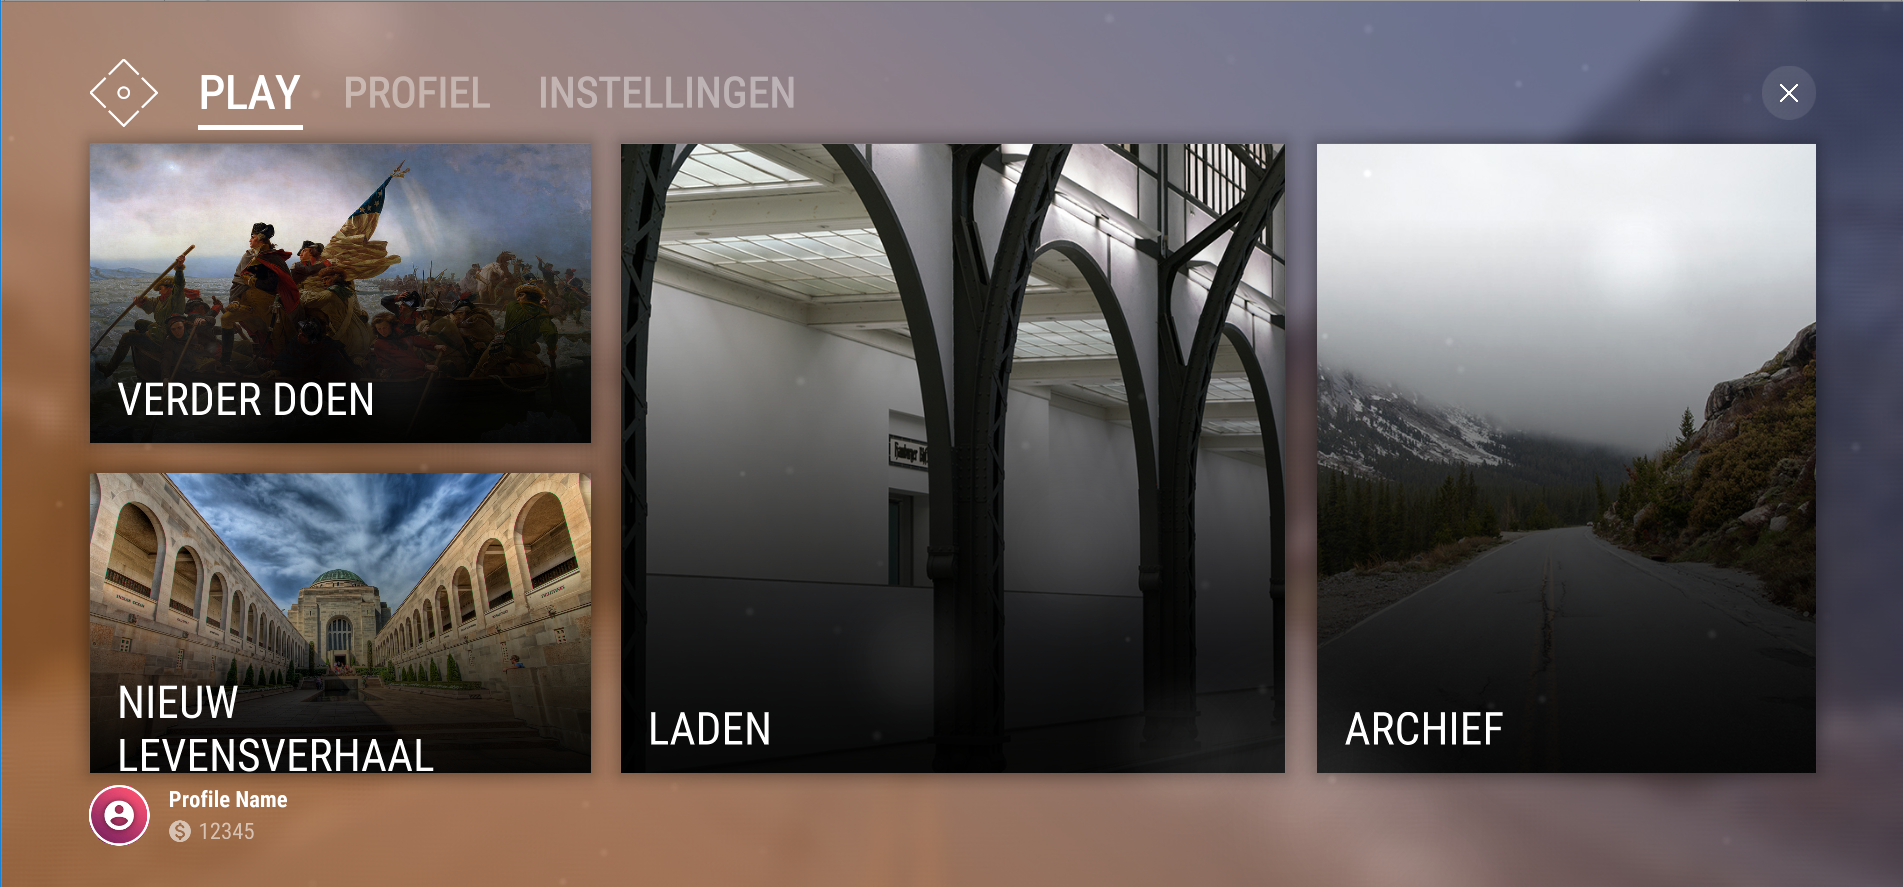
\includegraphics[width=\linewidth]{prototypeUi.png}
    \caption{Het hoofdmenu}
    \label{fig:prototypeUi}
\end{figure}
% + 1 If you get the reference

\section{Nieuw Levensverhaal Starten}
De gebruiker heeft de optie om een nieuw levensverhaal op te starten. Wanneer hij voor deze opties kiest krijgt hij een lijst van alle beschikbare levensverhalen. Deze lijst is niet hardcoded in de applicatie. Bij het opstarten zal de applicatie de lijst ophalen van een backendserver. Wanneer de gebruiker kiest voor levensverhaal moet de applicatie wel nog de concrete data ophalen van dit levensverhaal. Deze data is van het JSON datatype en bevat:

\begin{enumerate}
    \item Informatie over het levensverhaal
    \item Raadsels gelinkt aan het levensverhaal
    \item De benodigde afbeeldingen
\end{enumerate}

Door het levensverhaal op deze manier op te slaan is het makkelijk voor musea om nieuwe verhalen te creëren via een webinterface en deze direct beschikbaar te stellen voor de gebruiker. Omdat de afbeeldingen niet op voorhand beschikbaar zijn moet ARCore data image database wel 'at runtime' creëren. Het toevoegen van een image 'at runtime' duurt ongeveer 30ms (wat niet lang is) en zolang het creëren van deze database op een ander thread gebeurt kan de gebruiker nog steeds de UI gebruiken.

\subsection{Verloop van een Levensverhaal}
Wanneer het levensverhaal geladen is kan de gebruiker aan de slag gaan. De gebruiker krijgt het eerste kunstwerk te zien dat hij moet inscannen. Bij het inscannen van het kunstwerk krijgt de gebruiker dan wat extra informatie over het kunstwerk en de persoon waarover het gaat. Ook krijgt hij het volgende kunstwerk te zien dat hij moet inscannen. Bij het inscannen van het volgende kunstwerk kunnen er nu meerdere dingen gebeuren:

\begin{enumerate}
    \item Het nieuwe kunstwerk is beschikbaar
    \item Het nieuwe kunstwerk is nog niet beschikbaar en de gebruiker moest eerst een raadsel oplossen
\end{enumerate}

In het eerste geval gaat de applicatie gewoon verder zoals bij het eerste kunstwerk. Bij het tweede geval moet de gebruiker iets extra doen om het volgende kunstwerk te kunnen scannen. Deze raadsels kunnen van verschillende vormen waaronder:

\begin{enumerate}
    \item Antwoorden van een vraag
    \item Opzoek gaan naar een item in een voorafgaand kunstwerk
    \item Opzoek gaan naar een item in het huidige kunstwerk
\end{enumerate}

Deze cyclus blijft verder gaan tot de gebruiker het hele levensverhaal heeft ontdekt.

\section{Lijst van Levensverhalen}
In dit scherm bevinden zich alle levensverhalen die ooit hebben bestaan zelf als de gebruiker er niet aan heeft meegedaan. Op deze manier gaat het werk van het museum nooit verloren. De gebruikers kunnen hier een levensverhaal selecteren en de informatie over de kunstwerken lezen. Ook is er de optie om zelf de schilderijen af te drukken waardoor de gebruikers ook de mogelijkheid hebben om bij hun thuis de tentoonstelling uit te voeren.